\documentclass[12pt]{ctexart}
\usepackage{amsmath,graphicx,textcomp,subfigure,indentfirst,ctex,color,float}
\usepackage{bm, mhchem}
\title{Lecture 9}
\author{赵思逸}

\date{2022年4月26日}

\newcommand{\refeq}[1]{式~(\ref{#1})}
\newcommand{\reffig}[1]{图~(\ref{#1})}
\begin{document}

\maketitle

\section{CMB的偶极各向异性(dipole anisotropy)}

光子数密度符合普朗克公式
\begin{equation}
    n_T\left(\nu\right) d\nu = \frac{8\pi \nu^2 /c^3}{e^\frac{h\nu}{k_BT}-1} d\nu
\end{equation}

我们求相空间的数密度。相空间(坐标和动量组成的参数空间)的粒子数量 $N\left(\boldsymbol{x},\boldsymbol{p}\right) d^3x d^3p$是守恒量, 其中$d^3x d^3p$是相空间的体积元,是 Lorentz 不变量, 因此$N\left(\boldsymbol{x},\boldsymbol{p}\right)$也是Lorentz不变量。

对于光子, $|\boldsymbol{p}|=E/c=h_{\mathrm{pl}} \nu/c$,则 $d^3p=4\pi |\boldsymbol{p}|^2 dp=4\pi h_{\mathrm{pl}}^3 \nu^2/c^3 d\nu$. 且对于光子, $N_\gamma(\boldsymbol{x},\boldsymbol{p})=N_\gamma\left(p\right) $

光子数一定,
\begin{equation}
    N_\gamma(p)d^3x d^3p = \frac{1}{2} n_T\left(\nu\right) d\nu d^3x
\end{equation}
其中1/2是因为光子有两种极化。

得到 
\begin{equation}
    N_\gamma(p) = \frac{1}{h_{\mathrm{pl}}^3} \frac{1}{e^\frac{pc}{k_B T}-1}
\end{equation}

地球(以下带$'$的是地球坐标系)相对 共动坐标系有一个相对运动速度
$v = \mathcal{O} \left(100 \mathrm{km/s}\right) $, 
此时相对论的速度参数
$\beta \equiv v/c\sim 10^{-3}$,
$\gamma \equiv \left(1-\beta^2\right)^{-\frac{1}{2}}\sim 1$. 
设地球上观测到的光子动量$\boldsymbol{p'}$与地球坐标系运动速度$\boldsymbol{v}$夹角是$\theta$,$|\boldsymbol{p}| =\gamma \left(1+\beta \cos \theta \right) |\boldsymbol{p^\prime}|$
则
\begin{equation}
    N_\gamma^\prime(p') = \frac{1}{h_{\mathrm{pl}}^3} \frac{1}{e^\frac{p'c}{k_B T'}-1}
\end{equation}
\begin{equation}
    T'\left(\theta\right) = \frac{T}{\gamma \left(1+\beta \cos \theta\right) } \simeq T\left(1-\beta \cos \theta\right) 
\end{equation}
可以观测到偶极各向异性,其中$\theta=0$时(光子从后方追上观察者),观测到的温度$T'$偏低,$\theta=\pi$时(光子迎面而来),观测到的温度$T'$偏高。

实际观测到的CMB偶极矩说明了地球相对于“CMB frame”有运动。
扣除这个偶极矩后,我们可以得到宇宙真实的密度起伏。


\section{大爆炸核合成 \\(Big Bang Nucleosynthesis, BBN)}

对于一种原子核,原子序数 $Z$,
原子质量数 $A$, 原子核质量$m$, 中子质量 $m_n$, 质子质量$m_p$.
束缚能
\begin{equation}
    B=Z m_p + (A-Z) m_n -m
\end{equation}
质子中子能量差 $Q=m_n-m_p = 1.293 \mathrm{~MeV}$,
氘核结合能 $B_D = 2.22 \mathrm{~MeV} $.
% 比结合能约为 $1.11 \mathrm{~MeV} $, 小于质子中子能量差,所以 

大爆炸核合成的预言:
\begin{itemize}
    \item[1.] 轻元素(H, He, 部分 Li, C)在大爆炸中合成。
    \item[2.] 定量预言 H, He, Li, C 的丰度。
\end{itemize}

质子和中子通过弱相互作用可以相互转化。
\begin{eqnarray}
    p+\bar{\nu} \leftrightarrow n + e^+ \\ 
    p + e^- \leftrightarrow n + \nu \\ 
    n \leftrightarrow p + e^- + \bar{\nu}
\end{eqnarray}

% 第一步,“形成”更多的中子。
当温度降低到 $T\sim 0.1 \mathrm{~MeV}$ 时,反应向产生中子的一端移动, 质子转化成中子。
中子足够多后(当$T\sim 0.07 \mathrm{~MeV}$)就可以形成轻元素。
\begin{eqnarray}
    p+n \leftrightarrow D + \gamma \\ 
    D + D \leftrightarrow \ce{^{3}He} + n \\ 
    \ce{^{3}He} + D \leftrightarrow \ce{^{4}He} + p  
\end{eqnarray}

% 中微子 abundance 【【??】】

考虑 $T > 0.5 \mathrm{~MeV}$,% 光子、中微子、正负电子均为相对论性
平衡态方程
\begin{equation}
    \frac{n_p}{n_n} = \frac{n_p^{(0)}}{n_n^{(0)}} = e^\frac{Q}{k_B T}
\end{equation}

定义
$X_n\equiv \frac{n_n}{n_b} = \frac{n_n}{n_n+n_p}$,
即
\begin{equation}
    \frac{1-X_n}{X_n} = \frac{n_p}{n_n} = e^\frac{Q}{k_B T}
\end{equation}

反应发生后需要使用非平衡态的Boltzmann方程,
\begin{equation}
    \frac{dX_n}{dt} = \lambda_{np} \left( \left(1-X_n\right) e^{-\frac{Q }{k_B T}}-X_n\right) 
\end{equation}

其中速率 $\lambda_{np} = \frac{255}{\tau_n x^5} \left(12+6x+x^2\right) $,  
$x=\frac{Q}{k_B T}$.
当$T\simeq 0.5 \mathrm{~MeV}$时,
$X_n \simeq 0.15$,
中子寿命$\tau_n \simeq 15\mathrm{min} \simeq 886.7 \mathrm{sec}$.

轻元素形成时,温度$T_\text{nuc}\sim 0.07 \mathrm{~MeV}$, 
\begin{equation}
    X_n\left(T_\text{nuc}\right) = 0.15 \exp\left(-\frac{t }{\tau_n}\right) =0.11
\end{equation}

BBN时期的宇宙辐射占主导,$t\propto a^2\propto T^{-2}$.
\begin{equation}
    t = 132 \mathrm{sec} \left(\frac{0.1 \mathrm{~MeV}}{T}\right)^2 =   132 \mathrm{sec} \left(\frac{0.1 }{0.07}\right)^2 \simeq 269 \mathrm{sec}
\end{equation}

\begin{figure}[!hbtp]
	\centering
	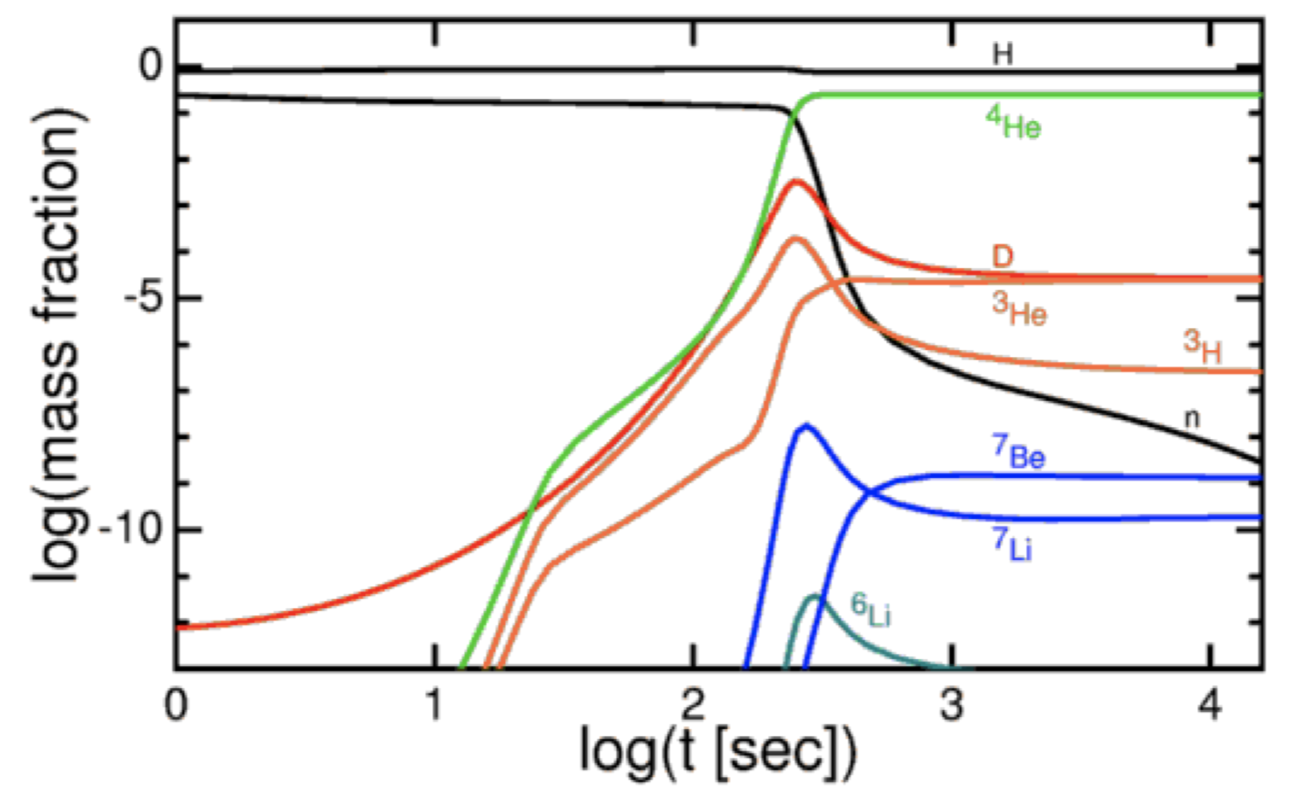
\includegraphics[width=1.0\linewidth]{BBNt.png}
	\caption{轻元素丰度随时间的变化(图源Hannu Kurki-Suonio)} \label{fig:BBNt}
\end{figure}

BBN期间各种原子核质量占比随时间的演化如 \reffig{fig:BBNt}   所示,可以看到BBN结束时,
多数中子都进入了$\ce{^{4}He} $, $X_{\ce{^{4}He} } \equiv \frac{4 n_{\ce{^{4}He} }}{n_b} = 2X_n\left(T_\text{nuc}\right) =0.22$.
这是估算,精确的结果是
\begin{equation}
    X_{\ce{^{4}He} } = 0.2262+0.0135 \ln \left( \frac{\eta_b}{10^{-10}}\right) \approx 0.24
\end{equation}
其中$\eta_b = \frac{n_b}{n_\gamma} \simeq 4\times 10^{-10}$, 与 $\Omega_b h^2$有关。

如果忽略掉质子和中子质量微小的差异,
那么$X_{\ce{^{4}He}}$的物理意义就是氦4的质量丰度,
有时候用$Y_p$表示,即氦4核在所有核子里的质量比。
此外,也经常定义以数量计算的氦4丰度 $y_{\ce{^{4}He}}$,即氦4核在所有原子核里的数量比。
由于氢(H)原子核只包含1个核子,而氦4($\ce{^{4}He}$)原子核包含4个核子,所以\\
\begin{equation}
    y_{\ce{^{4}He}} = \frac{ \frac{1}{4} X_{\ce{^{4}He}}}{ (1- X_{\ce{^{4}He}}) +  \frac{1}{4} X_{\ce{^{4}He}} } \approx 0.0724
\end{equation}

\begin{figure}[!hbtp]
	\centering
	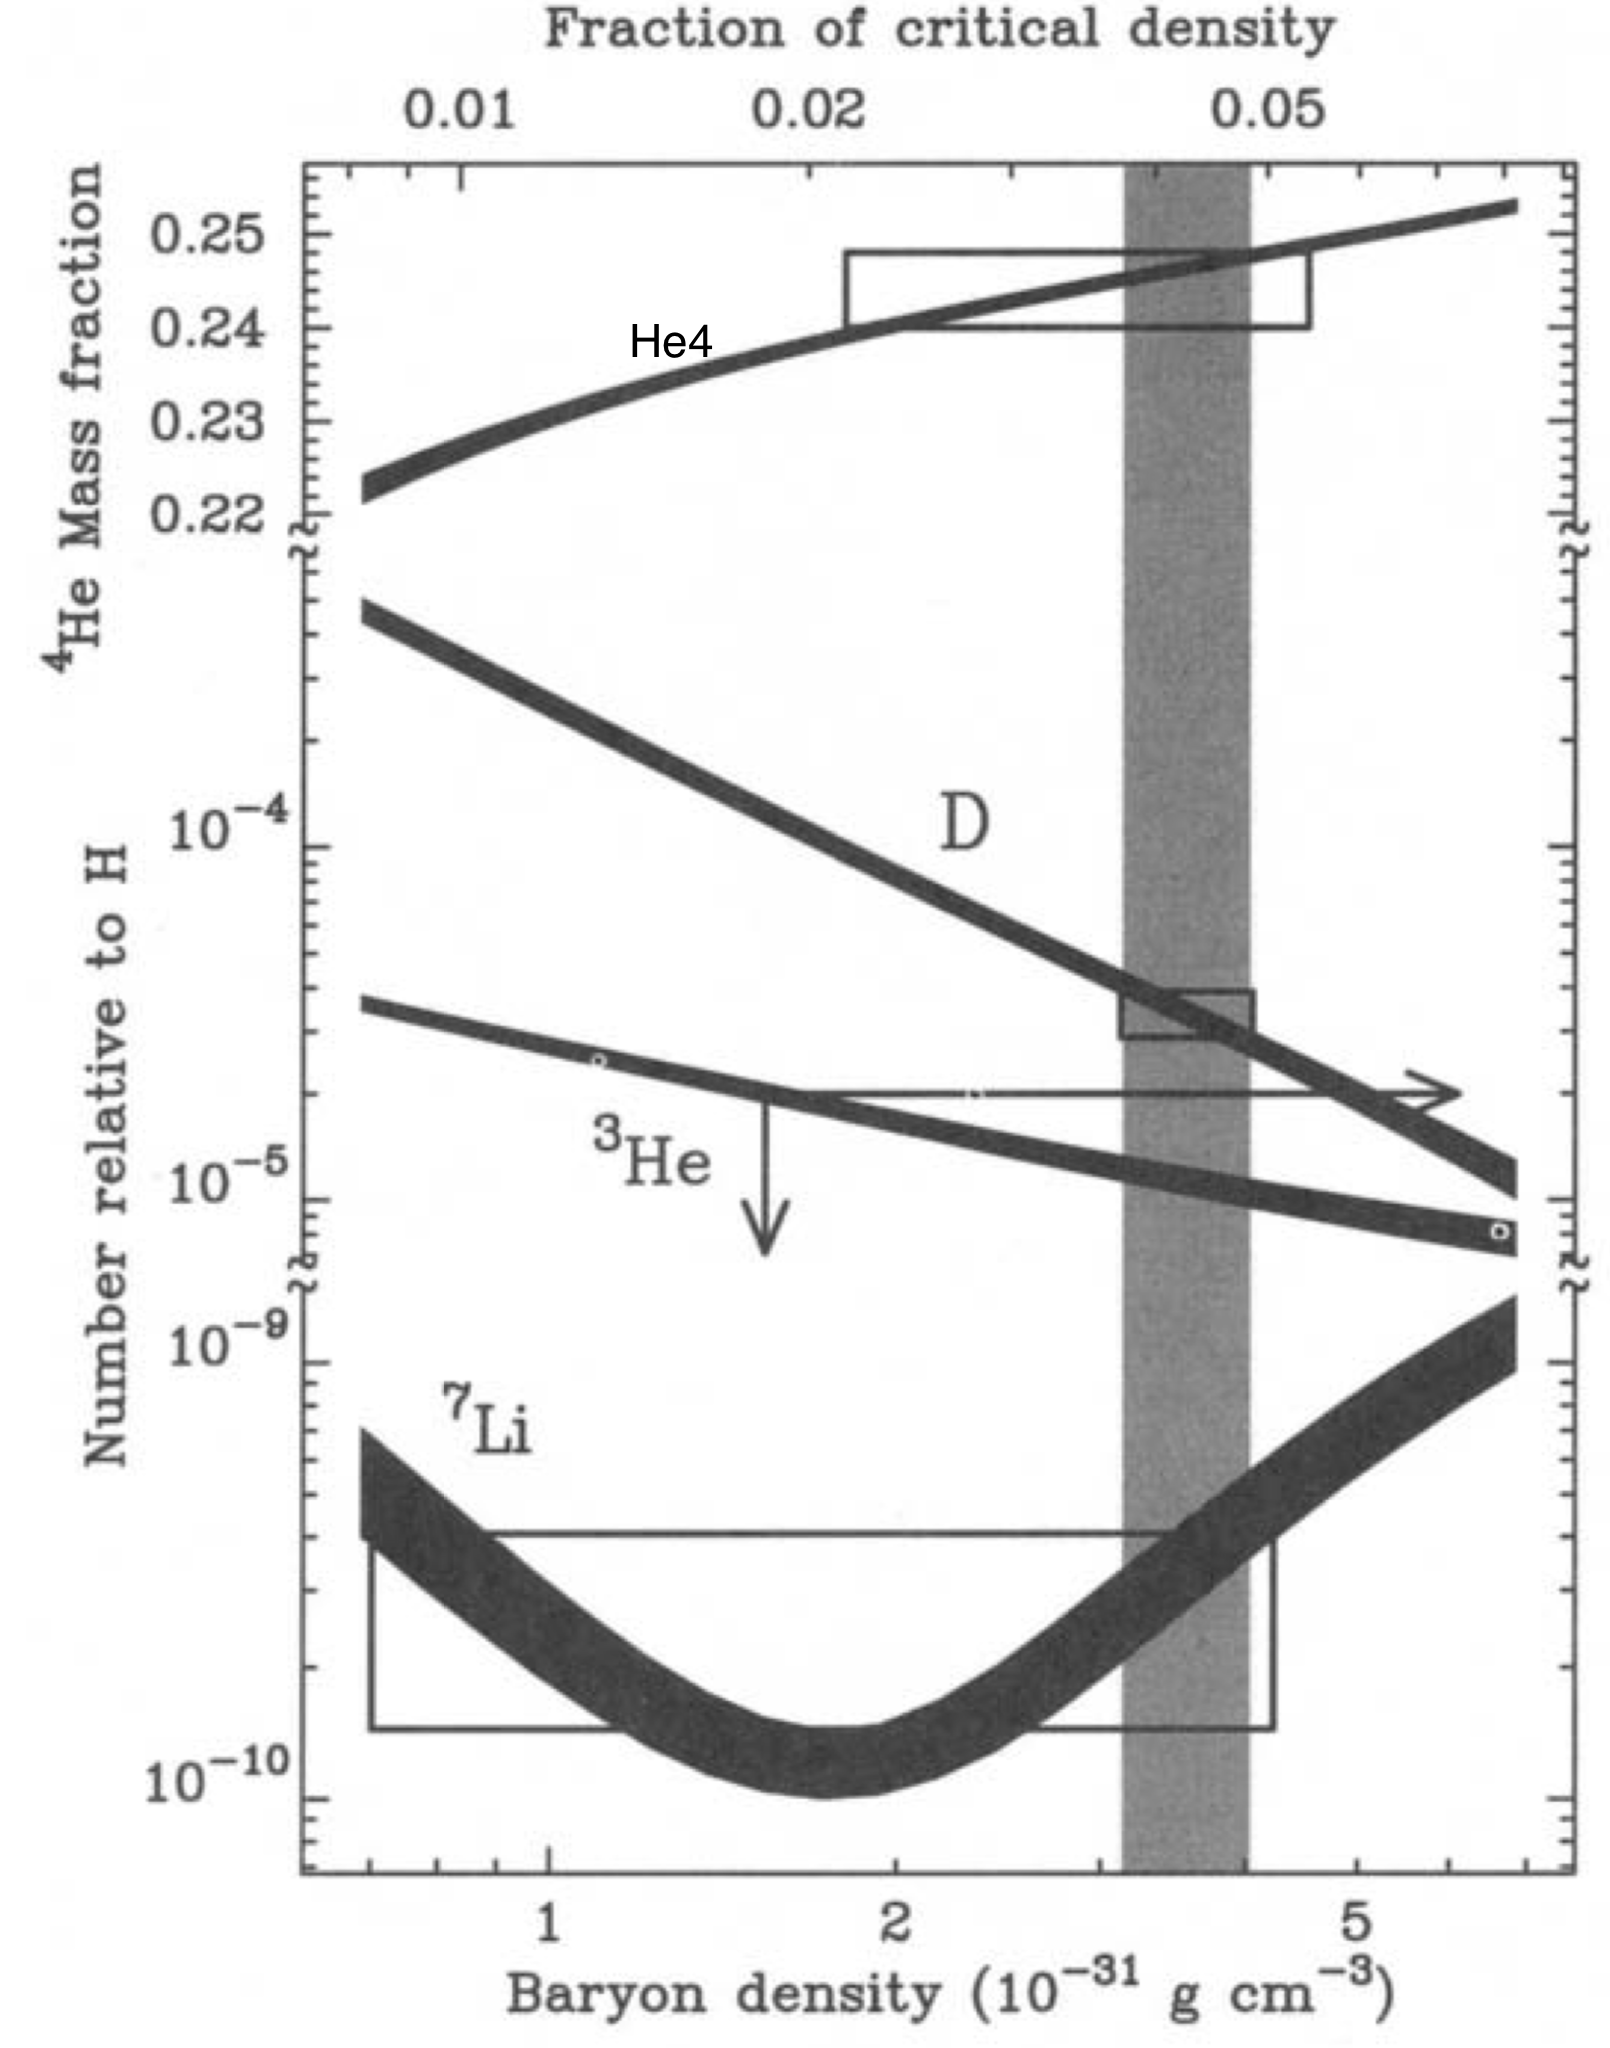
\includegraphics[width=1.0\linewidth]{BBN.png}
	\caption{轻元素丰度的预言和测量(图源Dodelson)} \label{fig:BBN}
\end{figure}

对BBN的测量见 \reffig{fig:BBN}。
从4个独立丰度测量得到自洽的 $\Omega_b h^2$ 限制。
\begin{eqnarray}
    \Omega_b \simeq 0.05 \\ 
    h\simeq 0.7 \\ 
    \Omega_b h^2 \simeq 0.025
\end{eqnarray}

\end{document}
